
%%%%%%%%%%%%%%%%%%%%%%%%%%%%%%%%%%%%%%%%%%%%%%%%%%%%%%%%%%%%%%%%%%%%%%%%%%%%%%%%%%%%%%%
%%%%%%%%%%%%%%%%%%%%%%%%%%%%%%%%%%%%%%%%%%%%%%%%%%%%%%%%%%%%%%%%%%%%%%%%%%%%%%%%%%%%%%%
% 
% This top part of the document is called the 'preamble'.  Modify it with caution!
%
% The real document starts below where it says 'The main document starts here'.

\documentclass[12pt]{article}

\usepackage{amssymb,amsmath,amsthm}
\usepackage[top=1in, bottom=1in, left=1.25in, right=1.25in]{geometry}
\usepackage{fancyhdr}
\usepackage{enumerate}
\usepackage{listings}
\usepackage{graphicx}
\usepackage{float}

\usepackage{mwe}
\usepackage{caption}
\usepackage{subcaption}
% Comment the following line to use TeX's default font of Computer Modern.
\usepackage{times,txfonts}



\makeatletter
\renewcommand*\env@matrix[1][*\c@MaxMatrixCols c]{%
  \hskip -\arraycolsep
  \let\@ifnextchar\new@ifnextchar
  \array{#1}}
\makeatother

\newtheoremstyle{homework}% name of the style to be used
  {18pt}% measure of space to leave above the theorem. E.g.: 3pt
  {12pt}% measure of space to leave below the theorem. E.g.: 3pt
  {}% name of font to use in the body of the theorem
  {}% measure of space to indent
  {\bfseries}% name of head font
  {:}% punctuation between head and body
  {2ex}% space after theorem head; " " = normal interword space
  {}% Manually specify head
\theoremstyle{homework} 

% Set up an Exercise environment and a Solution label.
\newtheorem*{exercisecore}{Exercise \@currentlabel}
\newenvironment{exercise}[1]
{\def\@currentlabel{#1}\exercisecore}
{\endexercisecore}

\newcommand{\localhead}[1]{\par\smallskip\noindent\textbf{#1}\nobreak\\}%
\newcommand\solution{\localhead{Solution:}}

%%%%%%%%%%%%%%%%%%%%%%%%%%%%%%%%%%%%%%%%%%%%%%%%%%%%%%%%%%%%%%%%%%%%%%%%
%
% Stuff for getting the name/document date/title across the header
\makeatletter
\RequirePackage{fancyhdr}
\pagestyle{fancy}
\fancyfoot[C]{\ifnum \value{page} > 1\relax\thepage\fi}
\fancyhead[L]{\ifx\@doclabel\@empty\else\@doclabel\fi}
\fancyhead[C]{\ifx\@docdate\@empty\else\@docdate\fi}
\fancyhead[R]{\ifx\@docauthor\@empty\else\@docauthor\fi}
\headheight 15pt

\def\doclabel#1{\gdef\@doclabel{#1}}
\doclabel{Use {\tt\textbackslash doclabel\{MY LABEL\}}.}
\def\docdate#1{\gdef\@docdate{#1}}
\docdate{Use {\tt\textbackslash docdate\{MY DATE\}}.}
\def\docauthor#1{\gdef\@docauthor{#1}}
\docauthor{Use {\tt\textbackslash docauthor\{MY NAME\}}.}
\makeatother

% Shortcuts for blackboard bold number sets (reals, integers, etc.)
\newcommand{\Reals}{\ensuremath{\mathbb R}}
\newcommand{\Nats}{\ensuremath{\mathbb N}}
\newcommand{\Ints}{\ensuremath{\mathbb Z}}
\newcommand{\Rats}{\ensuremath{\mathbb Q}}
\newcommand{\Cplx}{\ensuremath{\mathbb C}}
%% Some equivalents that some people may prefer.
\let\RR\Reals
\let\NN\Nats
\let\II\Ints
\let\CC\Cplx
%%%%%%%%%%%%%%%%%%%%%%%%%%%%%%%%%%%%%%%%%%%%%%%%%%%%%%%%%%%%%%%%%%%%%%%%%%%%%%%%%%%%%%%
%%%%%%%%%%%%%%%%%%%%%%%%%%%%%%%%%%%%%%%%%%%%%%%%%%%%%%%%%%%%%%%%%%%%%%%%%%%%%%%%%%%%%%%
% 
% The main document start here.

% The following commands set up the material that appears in the header.




%  \textbf{Code:}
%  \begin{center}
%  \lstinputlisting[basicstyle = \footnotesize]{}
%  \end{center}
%  
%  \begin{footnotesize}
%  \begin{verbatim}
%    
%  \end{verbatim}
%  \end{footnotesize}
%  
%  
%  \begin{figure}[H]
%    \begin{center}
%      \caption{}
%    \includegraphics[width = \textwidth]{}
%    \end{center}
%  \end{figure}




\doclabel{Stat 461: Homework 8}
\docauthor{Stefano Fochesatto}
\docdate{\today}

\begin{document}
\begin{exercise}{1} The idea of credit scorning is that you try to classify people into a group that will pay the money back and a group that won't. We'll use a version of a well-known dataset called Kredit, 
  which contained data from 1000 germans. This version we'll use is from kaggle.\\
  \begin{enumerate}
    \item[a.] Load the csv german\_credit\_data.\\
    \solution Reading in the data we find that the checking and saving account variables contain all the missing values. Simply removing all the rows with missing values reduces our number of observations to 522, which is about half.
    I am not necessary sure we should be throwing out so much of our data, for two variables which are not entirely indicative of an individuals credit responsibility. There are a few actions we can take to try and save this data.
    We could impute the medium value for these missing values, use a discriminant method that is robust to missing values like decision trees, or we could simply drop these categorical predictors. I ended up deciding to remove the variables.\\
      \textbf{Code:}
      \begin{center}
      \lstinputlisting[basicstyle = \footnotesize]{r1.txt}
      \end{center}
      \vspace{.15in}

    \item[b.] Try a k-nearest neighbors classification. Select a value of k that you think is reasonable, then split the data into a training set and a testing set, then look at how well it classified the test data.\\
    \solution From the data set we know that there are likely only two groups represented in the data. We can verify this by simulating kmeans clusters and computing the rsquared between them. Doing so we found that $k = 2$
    is explaining a majority of the variance. Using a 80/20 split for training testing data we found that the kmeans clustering performed rather poorly, misclassifying 86 of the 200 testing data achieving an accuracy of 57\%.
      \begin{figure}[H]
        \begin{center}
          \caption{Proportion of rSquared for each K.}
        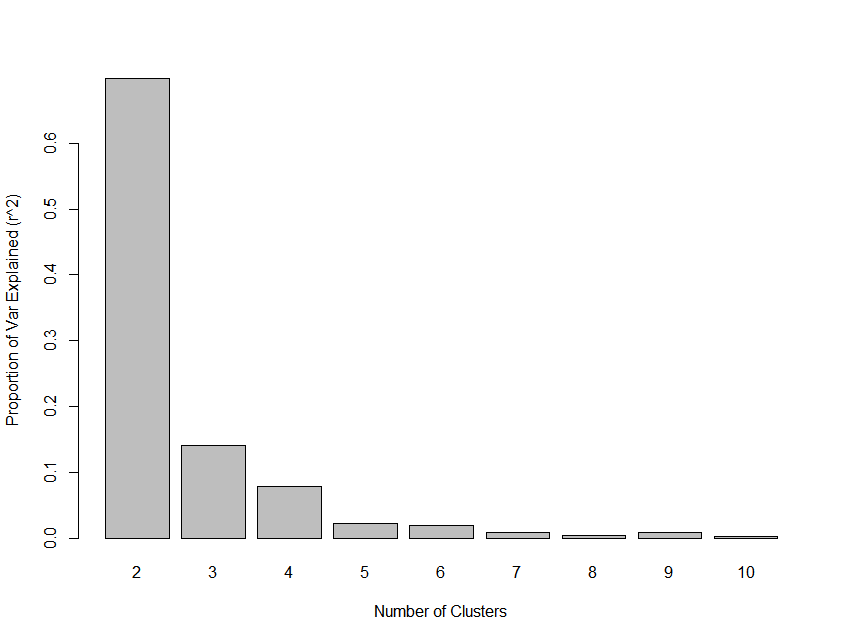
\includegraphics[width = \textwidth]{Rplot01.png}
        \end{center}
      \end{figure}
        \textbf{Code:}
        \begin{center}
        \lstinputlisting[basicstyle = \footnotesize]{r2.txt} 
        \end{center}
        \vspace{.15in}

    \item[c.] Now repeat (b), but this time perform a cross validation. Which of these confusion matrices do you think gives you a better idea as to how well KNN will classify new observations.\\ 
    \solution Applying one-out cross validation we get that the KNN misclassified 509 of the 1000 observations achieving an accuracy of 49\%.
    Generally I will tend to trust the more skeptical model validation method so in this case I think the $\sim 50\%$ accuracy is true to what the KNN model is doing. Ideally we would be training the model on all the data, 
    and gather more data to validate the model, rather than doing a split or cross validation.  \\
    \textbf{Code:}
    \begin{center}
    \lstinputlisting[basicstyle = \footnotesize]{r3.txt} 
    \end{center}
    \vspace{.15in}

    \item[d.] Try several values of $k$ and look at the test/trina confusion matrix from (b) for each value of $k$. What is your preferred value of $k$.\\
    \solution   
  
  
  
      \end{enumerate}

\end{exercise}





\end{document}


















